%% The '3p' and 'times' class options of elsarticle are used for Elsevier CRC
%% The 'procedia' option causes ecrc to approximate to the Word template
\documentclass[3p,times,procedia]{elsarticle}
\flushbottom

%% The `ecrc' package must be called to make the CRC functionality available
\usepackage{ecrc}
\usepackage[colorlinks=true]{hyperref}%url}
\usepackage{amsmath}


%% The ecrc package defines commands needed for running heads and logos.
%% For running heads, you can set the journal name, the volume, the starting page and the authors

%% set the volume if you know. Otherwise `00'
\volume{00}

%% set the starting page if not 1
\firstpage{1}

%% Give the name of the journal
\journalname{Physics Procedia}

%% Give the author list to appear in the running head
%% Example \runauth{C.V. Radhakrishnan et al.}
\runauth{A. E. Antipov et al.}

%% The choice of journal logo is determined by the \jid and \jnltitlelogo commands.
%% A user-supplied logo with the name <\jid>logo.pdf will be inserted if present.
%% e.g. if \jid{yspmi} the system will look for a file yspmilogo.pdf
%% Otherwise the content of \jnltitlelogo will be set between horizontal lines as a default logo

%% Give the abbreviation of the Journal.
\jid{phpro}

%% Give a short journal name for the dummy logo (if needed)
\jnltitlelogo{Physics Procedia}


\usepackage{amssymb}
%% The amsthm package provides extended theorem environments
%% \usepackage{amsthm}

%% The lineno packages adds line numbers. Start line numbering with
%% \begin{linenumbers}, end it with \end{linenumbers}. Or switch it on
%% for the whole article with \linenumbers after \end{frontmatter}.
%% \usepackage{lineno}

%% natbib.sty is loaded by default. However, natbib options can be
%% provided with \biboptions{...} command. Following options are
%% valid:

%%   round  -  round parentheses are used (default)
%%   square -  square brackets are used   [option]
%%   curly  -  curly braces are used      {option}
%%   angle  -  angle brackets are used    <option>
%%   semicolon  -  multiple citations separated by semi-colon
%%   colon  - same as semicolon, an earlier confusion
%%   comma  -  separated by comma
%%   numbers-  selects numerical citations
%%   super  -  numerical citations as superscripts
%%   sort   -  sorts multiple citations according to order in ref. list
%%   sort&compress   -  like sort, but also compresses numerical citations
%%   compress - compresses without sorting
%%
\biboptions{authoryear}

% \biboptions{}

% if you have landscape tables
\usepackage[figuresright]{rotating}
%\usepackage{harvard}
% put your own definitions here:x
%   \newcommand{\cZ}{\cal{Z}}
%   \newtheorem{def}{Definition}[section]
%   ...

% add words to TeX's hyphenation exception list
%\hyphenation{author another created financial paper re-commend-ed Post-Script}

% declarations for front matter

\begin{document}

\begin{frontmatter}

%% Title, authors and addresses

%% use the tnoteref command within \title for footnotes;
%% use the tnotetext command for the associated footnote;
%% use the fnref command within \author or \address for footnotes;
%% use the fntext command for the associated footnote;
%% use the corref command within \author for corresponding author footnotes;
%% use the cortext command for the associated footnote;
%% use the ead command for the email address,
%% and the form \ead[url] for the home page:
%%
%% \title{Title\tnoteref{label1}}
%% \tnotetext[label1]{}
%% \author{Name\corref{cor1}\fnref{label2}}
%% \ead{email address}
%% \ead[url]{home page}
%% \fntext[label2]{}
%% \cortext[cor1]{}
%% \address{Address\fnref{label3}}
%% \fntext[label3]{}

\dochead{28th Annual CSP Workshop on ``Recent Developments in Computer Simulation Studies in Condensed Matter Physics'', CSP 2015}
%% Use \dochead if there is an article header, e.g. \dochead{Short communication}
%% \dochead can also be used to include a conference title, if directed by the editors
%% e.g. \dochead{17th International Conference on Dynamical Processes in Excited States of Solids}

\title{OpenDF - a multiscale method for strongly correlated systems }

%% use optional labels to link authors explicitly to addresses:
%% \author[label1,label2]{<author name>}
%% \address[label1]{<address>}
%% \address[label2]{<address>}



\author[a]{Andrey E. Antipov\corref{cor1}} 
\author[a]{James P.F. LeBlanc}
\author[a]{Emanuel Gull}

\address[a]{Department of Physics, University of Michigan, Ann Arbor, Michigan 48109, USA}

\begin{abstract}
We present the new open-source algorithm, \textbf{opendf} code -  a multiscale approach, that utilizes recently developed dual fermion method, to solve lattice problems of interacting strongly correlated systems. In particular, the present distribution of the code provides an approximate solution for the ubiquitous Hubbard model in various dimensions $d=1,2,3,4$. The method is designed to be the ending step of the self-consistency procedure of dynamical mean field theory (DMFT) and hence utilizes the DMFT input: Green's function and full reducible vertex functions. As an output the code provides spatially dependent susceptibilities and Green's functions of the model. The package is distributed as an open-source package. 
\end{abstract}

\begin{keyword}
Type your keywords here, separated by semicolons ; 

%% keywords here, in the form: keyword \sep keyword

%% PACS codes here, in the form: \PACS code \sep code

%% MSC codes here, in the form: \MSC code \sep code
%% or \MSC[2008] code \sep code (2000 is the default)

\end{keyword}
\cortext[cor1]{Corresponding author.}
\end{frontmatter}

%\correspondingauthor[*]{Corresponding author. Tel.: +0-000-000-0000 ; fax: +0-000-000-0000.}
\email{aantipov@umich.edu}

%%
%% Start line numbering here if you want
%%
% \linenumbers

%% main text

%\enlargethispage{-7mm}
\vspace*{-8pt}
\section{Introduction}
The task of a reliable description of interacting many-body quantum systems is of a paradigmatic importance. 
Correlations between multiple particles is a driving force behind many of ubiquitous phenomena in modern condensed matter science, including high-temperature superconductivity ... 
\section{Solved equations}
text text text
\section{Implementation and examples}

\begin{figure}[ht]
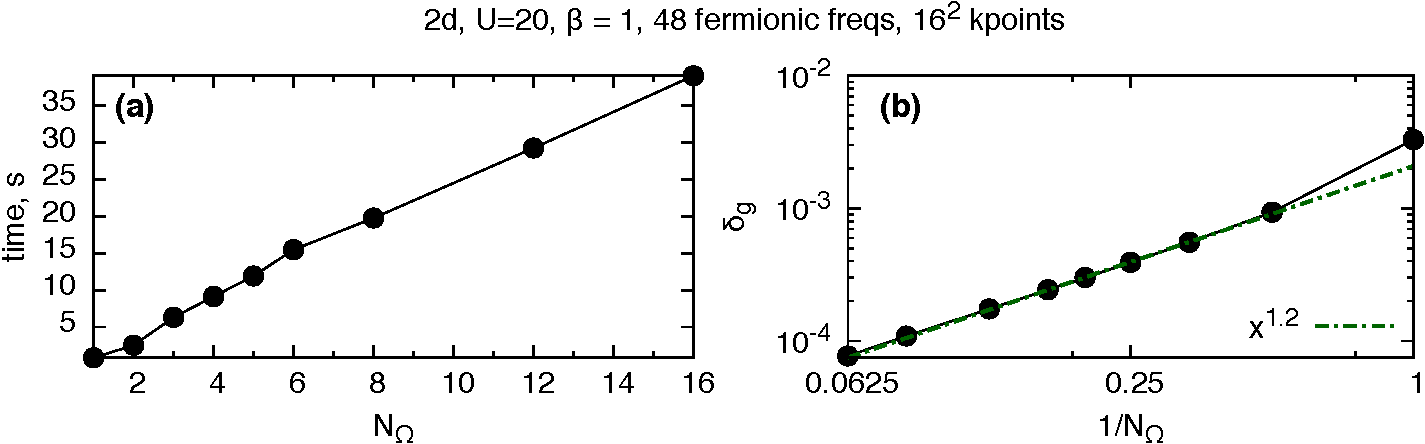
\includegraphics[width=0.5\columnwidth]{time_bfreqs.pdf}
\caption{Bosonic scaling}
\end{figure}

\begin{figure}[ht]
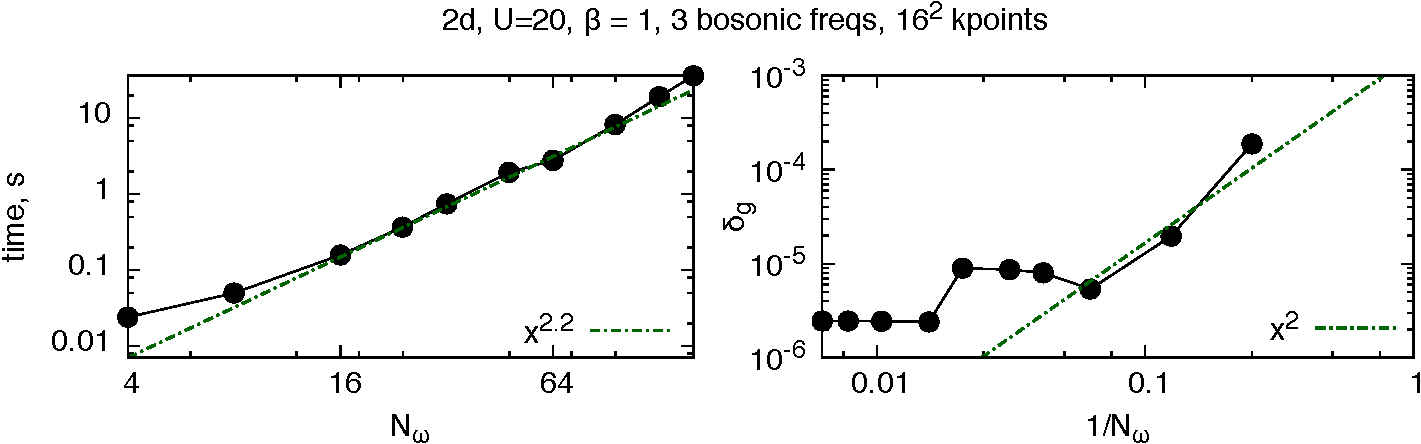
\includegraphics[width=0.5\columnwidth]{time_ffreqs.pdf}
\caption{Fermionic scaling}
\end{figure}

\begin{figure}[ht]
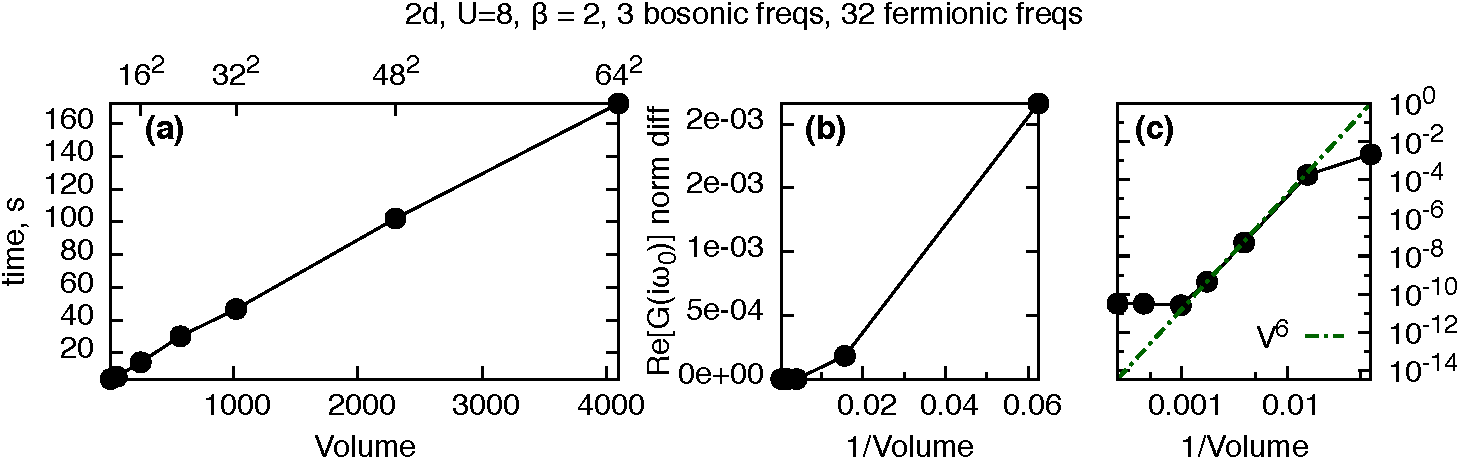
\includegraphics[width=0.5\columnwidth]{time_kpts.pdf}
\caption{Volume scaling}
\end{figure}


\section{Conclusion}
text text text


\section*{Acknowledgements}
Acknowledgements 

\end{document}


